% Identity-free manuscript prepared for external scientific review.
% Author-identifying and author-controlled submission fields are withheld until explicitly approved.
\documentclass[10pt]{article}

\usepackage[a4paper,margin=0.82in]{geometry}
\usepackage{amsmath,amssymb,amsthm}
\usepackage{array}
\usepackage{booktabs}
\usepackage{graphicx}
\usepackage{float}
\usepackage[hidelinks]{hyperref}
\hypersetup{
  pdftitle={Exact reversible choice coding with retrospective assay-guided selection in PCR-tested oligonucleotide libraries},
  pdfsubject={Anonymous Bioinformatics methods manuscript},
  pdfkeywords={DNA data storage, constrained coding, assay calibration, PCR efficiency, reversible coding}
}

\newtheorem{proposition}{Proposition}
\newcommand{\DNA}{\{A,C,G,T\}}
\emergencystretch=2em

\title{Exact reversible choice coding with retrospective assay-guided selection in PCR-tested oligonucleotide libraries}
\author{}
\date{}

\begin{document}
\maketitle

\begin{abstract}
\noindent\textbf{Motivation:} DNA-storage design requires exact payload inversion while allowing assay-specific sequence ranking.

\noindent\textbf{Results:} We assign each payload $2^r$ valid candidates; a deterministic assay scorer selects one, whereas exact modulo-$|\mathcal C|$ inversion recovers the payload from any candidate without the scorer, at an $r$-bit cost. Retrospective PCR-tested GCall/GCfix codebooks gave $r=2$ measured selected-minus-fiber-mean gains of 0.250 and 0.274 target SDs. An outcome-blind 2,048-sequence external-laboratory KAPA codebook drawn from 9,995 already-public measurements in the same source publication gave 0.229--0.390 SD gains; 17.2--30.9\% of matched-condition fibers had negative gain. Comparisons with released 1D-CNN outputs were endpoint-dependent, and a secondary exploratory Q5 analysis reversed direction. All 65,024 generated candidates round-tripped; gains were predicted and none was synthesized or assayed. Reversibility is model- and assay-independent; utility is assay-dependent.

\noindent\textbf{Availability and implementation:} Code and frozen outputs: \url{https://github.com/nessajzhang/exact-reversible-choice-coding} (BSD-3-Clause).\\
\textbf{Contact:} Withheld.\\
\textbf{Supplementary information:} Available.
\end{abstract}

\section{Introduction}

Exact constrained coding has a long history in enumerative and finite-state source coding \cite{cover1973enumerative,adler1983slidingblock}. DNA-storage implementations now provide reversible GC-, homopolymer- and motif-constrained maps, including block and arithmetic constructions \cite{wang2019bioconstrained,immink2019balancedhomopolymer,welzel2023dnaaeon,ruan2026scone}. Candidate screening is also established: DNA Fountain discards seeds that generate unsuitable oligonucleotides, while DNA Chisel and RNAblueprint expose flexible sequence-optimization or constrained-sampling interfaces \cite{erlich2017dnafountain,zulkower2020dnachisel,hammer2017rnablueprint}. More generally, trellis shaping selects a representative from an equivalence class, and list-encoding distribution matching generates semantically equivalent candidates for metric-based selection \cite{forney1992trellisshaping,wu2022listccdm}. Neither reversible constraint control nor representative selection is therefore a broad novelty claim.

The narrower problem is the interface between exact payload semantics and an empirical assay utility. Multi-template PCR can produce sequence-specific amplification differences that depend on adapters, polymerase and the complete construct \cite{gimpel2025pcrbias}. Such a utility may be learned from experimental data, need not be finite-state and need not correspond to a free-energy model. Post hoc optimization can alter the payload, whereas threshold rejection can fail at a fixed candidate cap. A useful interface should admit an arbitrary deterministic selector, preserve a transparent payload inverse and charge a fixed rate cost.

We instantiate a fixed-rate shaping/list-selection interface as \emph{choice fibers}. An exact oligonucleotide codec assigns each payload $2^r$ valid candidates. A frozen assay model chooses the highest-scoring representative; the payload decoder ranks the received sequence exactly within the constrained language, inverts a full-language permutation and removes the $r$ selector bits. The methodological increment is the following combination rather than rank/unrank, affine permutation or representative selection alone: a globally defined exact map; fixed, disjoint $2^r$-member fibers; an exact $r$-bit rate cost; an arbitrary deterministic assay-specific selector; payload inversion that neither stores nor executes that selector; scorer replacement without loss of historical decodability; separation of payload recovery from optional canonical-output verification; and identical-fiber comparison of selectors against real PCR measurements. These properties decouple coding correctness from empirical score validity.

Five evidence types are kept distinct. Bidirectional GCall/GCfix codebooks provide retrospective measured cross-pool selection. A dated analysis plan applied before local scoring evaluates the frozen source models in an external-laboratory KAPA pool of already-public measurements reported in the same source publication; this is neither prospective preregistration nor independent third-party replication. A secondary exploratory Q5 analysis is an altered-protocol measured evaluation. A generated 108-nt language provides exact computational verification and model-predicted score diagnostics only. Prospective synthesis and PCR of codec-emitted codewords were not performed. The study therefore supports retrospective measured selection plus an exact computational codec interface, not prospective emitted-codeword benefit, mechanism, material recovery or end-to-end storage superiority.

\section{System and methods}

\subsection{Assay data, roles and selectors}

We used the public multi-template PCR data of Gimpel \emph{et al.} \cite{gimpel2025pcrbias}: 11,998 GCall and 11,994 GCfix variable sequences (108 nt) with measured relative amplification efficiency. Each was reconstructed as the assayed 149-nt construct using the published 20-nt left and 21-nt reverse-complemented right adapters. The sequence was the independent unit. Standardized ridge models used $\alpha\in\{10^{-4},\ldots,10^4\}$; within-pool estimates used five repeats of nested five-fold cross-validation, with scaling and penalty selection confined to each outer training fold. Source-only transfer fitted one complete source pool and ranked another without its outcomes.

Three nested selectors were compared on identical fibers. Composition (P0) used nucleotide frequencies, absolute GC deviation and maximum homopolymer length. AssayContext (P2) added variable-region candidate-pair and longest-stem features plus eight adapter-boundary features. FullContext (P5) added weighted pair counts and candidate-count/longest-stem features from the complete oligonucleotide. The exploratory feature ladder is defined in Supplementary Information; only P0, P2 and P5 entered the selector benchmark. The fitted score $u_z(x)$ is an assay-context ranking function, not a calibrated probability, free energy or mechanistic model.

Bidirectional GCall/GCfix evaluation was retrospective cross-pool transfer, not a permanent lockbox: target outcomes were excluded from source fitting, target membership, ordering and fiber assignment, but each pool served as source in one direction. The same-publication external-laboratory release contained 10,000 random sequences after motif-inserted sequences were excluded; 9,995 had measured efficiency under KAPA SYBR FAST at $54\,^{\circ}$C (``external KAPA''). The unchanged codec-eligibility rule left 2,053 sequences, and an outcome-blind SHA-256 order fixed a 2,048-sequence codebook. The measurements were already public; before local scoring and evaluation, a dated analysis plan fixed the endpoint, hash key, library, primary $r=2$ and secondary $r=4$ settings, selectors, estimand and resampling. This was an outcome-blind analysis lock, not prospective preregistration. Both source models were retained. Q5 Hot Start High-Fidelity at $60\,^{\circ}$C was identified as a workflow-shift endpoint, but its later Q5-complete codebook and missing-value implementation were not fully prespecified; Q5 is therefore secondary and exploratory. Dataset roles, assay conditions and sample counts are tabulated in Supplementary Table S5.

For fixed-length leakage control, we exhaustively compared the $143{,}904{,}012$ oriented GCall--GCfix pairs and each source against the external eligible/codebook sequences by Hamming distance, exact identity and reverse complement. Shared adapters were excluded because they were declared assay context. We did not audit edit-distance neighbourhoods, design-template genealogy or sequence-cluster independence; the result is a Hamming-separation audit, not proof of biological independence.

\subsection{Estimands and uncertainty}

The primary fiber contrast was selected measured efficiency minus the candidate mean. We report effect sizes, target-library standardization, fiber distributions and 2,000 target-fiber bootstrap intervals. Paired selector contrasts used the same fibers; an endpoint-matched secondary analysis compared selected low-efficiency events with fiber event rates. For FullContext, AssayContext and their contrasts, a two-stage bootstrap resampled original source-sequence IDs as integer weights, repeated scaling, penalty selection and fitting, and then resampled target fibers; all copies of a source sequence retained one fold from a fixed five-fold assignment, preventing bootstrap duplicates from crossing training and validation. Released CNN outputs remained fixed. Detailed randomization tests used 100,000 within-fiber draws and are reported only in Supplementary Information.

Intervals remain conditional on the published sequence-level outcome estimates and the final feature families, model class, endpoints, filters, codebook rules and mapping plans. They do not propagate technical-replicate, batch, normalization or assay-measurement uncertainty from the source experiments, or uncertainty from the complete exploratory research process. The external KAPA codebook was fixed by the dated plan before local scoring of already-public outcomes; bidirectional transfer, alternative mappings, Q5 implementation and abstention diagnostics are labelled retrospective or exploratory as applicable. No omnibus or universal superiority claim is made.

\section{Algorithm}

\subsection{Constrained language and full-language mapping}

Let
\[
 \mathcal C=\{x\in\DNA^{108}:49\leq\operatorname{GC}(x)\leq59,\ 
 \operatorname{HP}_{\max}(x)\leq3\}.
\]
Lexicographic completion counts use state $(t,g,b,h)$: remaining length $t$, current whole-sequence GC count $g$, last base $b$ and run length $h$. Exact integer branch masses define mutually inverse rank and unrank operations over $\mathcal C$. Independent top-down and bottom-up recurrences were required to agree. A reduced length-8 language was explicitly enumerated and every rank checked.

Let $N=|\mathcal C|=2.152086779\times10^{64}$ and $M=2^{213}$; the full integer $N$ is reported in Supplementary Information. Logical ranks use $0\leq q<M$, giving $K=213$ base bits and 1.9722 bits per variable-region nucleotide. All generated-code rates are normalized by the 108-nt variable region and exclude the fixed 41-nt adapters. To avoid confining codewords to the lexicographic prefix $[0,M)$, a fixed full-language affine map
\[
 R(q)=(aq+c)\bmod N,\qquad \gcd(a,N)=1,
\]
is a permutation of $[0,N)$ and therefore has an exact inverse. This number-theoretic property guarantees reversibility, but it does not guarantee useful within-fiber score, motif or structural diversity. The implemented $(a,c)$ was derived only from $N$ and a versioned SHA-256 namespace, without PCR outcomes, and was fixed before regenerated-language scoring. It is one admissible mapping, not an asserted optimum; eight independently derived namespaces provide empirical rank-spreading and score-sensitivity diagnostics.

\subsection{Reversible choice coding}

For selector width $r\leq K$ and payload $m\in\{0,\ldots,2^{K-r}-1\}$, define
\[
 q_{m,j}=m2^r+j,\qquad
 x_{m,j}=E\!\left(R(q_{m,j})\right),\qquad 0\leq j<2^r,
\]
where $E$ is the exact base unranker. The encoder emits $x_{m,j^\star}$ with
\[
 j^\star=\arg\max_j \kappa_z(x_{m,j}),\qquad
 \kappa_z(x)=\operatorname{RTE}\!\left(10^{12}u_z(x)\right),
\]
where RTE is round-to-nearest with ties to even, matching \texttt{numpy.rint} in the canonical reference implementation. Scores are binary64; non-finite values or rounded keys outside $[-2^{63},2^{63}-1]$ are rejected. The encoder lexicographically minimizes $(-\kappa_z,j)$, so equal keys select the smallest choice index. This quantization changed no AssayContext, FullContext or released-1D-CNN choice in the primary comparisons; four exploratory Composition choices changed, and the quantized results are frozen.

\begin{proposition}[Legal, fixed and disjoint fibers]
For every $0\leq r\leq K$ and valid payload $m$, $\mathcal F_m=\{x_{m,j}:0\leq j<2^r\}$ contains exactly $2^r$ members of $\mathcal C$. Fibers for distinct payloads are disjoint. If all candidate score keys are finite, encoding is total and deterministic.
\end{proposition}

\noindent
The logical intervals $[m2^r,(m+1)2^r)$ are disjoint subsets of $[0,M)$. The modulo-$N$ map and exact unranker are injective, so they preserve cardinality and disjointness; fixed-key maximization with the declared tie rule returns exactly one member.

\begin{proposition}[Score-independent payload inversion]
For every deterministic score $u_z$, the decoder
\[
 q=R^{-1}\!\left(D(x)\right)\bmod N,\qquad
 \operatorname{Dec}_{\rm payload}(x)=\left\lfloor q/2^r\right\rfloor
\]
returns $m$ for every candidate $x=x_{m,j}$, including the selected candidate, after rejecting $q\geq M$.
\end{proposition}

\noindent
Indeed, $D(E(R(q_{m,j})))=R(q_{m,j})$, inverse mapping returns $q_{m,j}<M$, and right shift by $r$ returns $m$. The exact rate is $(K-r)/108$ bits per variable-region nucleotide. The payload decoder accepts any valid candidate in the declared fiber. A separate optional $\operatorname{VerifyCanonical}_z$ may recompute the score and tie rule to accept only the representative that the encoder would emit; it is not part of payload inversion.

\begin{proposition}[Scorer-replacement invariance]
Replacing, upgrading or losing $u_z$ cannot change payload recovery for an existing valid candidate. It can change which representative a future encoder emits and whether the optional current-scorer verifier calls a historical candidate canonical.
\end{proposition}

\subsection{Algorithmic interface and failure behavior}

The generated-language encoder takes $(m,r,\text{codec namespace},u_z)$, checks $0\leq m<2^{K-r}$ and $0\leq r\leq K$, constructs all $q_{m,j}$ and $x_{m,j}$, requires finite score keys, applies the declared tie rule and returns one 108-nt codeword. No per-codeword score or choice-index metadata is required; the decoder needs only the versioned codec parameters and $r$. For a received sequence $x$, $\operatorname{Dec}_{\rm payload}$ checks length and the A/C/G/T alphabet, verifies membership in $\mathcal C$, computes $D(x)$, applies $R^{-1}$, rejects $q\geq M$, and returns $(m,j)=(q\mathbin{\mathrm{div}}2^r,q\bmod2^r)$. Wrong length, ambiguous bases, constraint violations and out-of-domain inverse ranks are rejected. Missing or replaced scores do not affect this path.

The optional $\operatorname{VerifyCanonical}_z$ reconstructs the decoded fiber, recomputes finite fixed-precision keys and checks that $x$ is the smallest-index maximizer. It is unavailable without the scorer and may reject a payload-decodable historical representative after a scorer change. Thus payload recovery and canonical verification are separate interfaces. The finite public-codebook analogue additionally requires a frozen codebook identifier; unknown sequences fail lookup. Detailed pseudocode, metadata requirements and tested failure cases are in Supplementary Information.

\section{Implementation}

\subsection{Finite experimental codebooks and comparators}

For each source--target setting, eligible target sequences were ordered by a SHA-256 key containing only a versioned namespace, direction and sequence hash. The first 2,048 sequences formed an outcome-blind 11-bit base codebook. Consecutive groups of $2^r$ sequences formed non-overlapping fibers; $r=2$ yielded 512 fibers and $r=4$ yielded 128. A selector fitted only in the source pool chose one sequence per fiber. Frozen-rank lookup and right shift defined $\operatorname{Dec}_{\rm payload}$ for any member of that fiber; an optional canonical verifier separately checked the selected representative. The resulting $11-r$ bits are a codebook index, not physical storage density.

The primary released state-of-the-art comparator was the original study's 1D-CNN output. On GCall/GCfix cross-pool fibers, candidate choice maximized the released 1D-CNN regression score. On the analysis-plan-locked external KAPA pool, candidate choice minimized the released 1D-CNN low-efficiency probability. These distinct objectives are named separately throughout and were not refitted by this study. A second cross-pool comparator reproduced the published hard rule, GC fraction between 0.4 and 0.6, homopolymer below 5 and mfold free energy above $-15$ kcal/mol, using the authors' released sequence-property table. Among passing candidates the smallest rank was chosen; a fiber without a passing candidate failed. We did not substitute another folding engine on the external pool.

\subsection{Generated-language and domain-boundary audits}

For each $r=0,\ldots,6$, 512 deterministic payloads were sampled from the fixed domain. All $2^r$ candidates were generated and reranked, producing 65,024 candidate checks. FullContext models fitted separately in GCall and GCfix selected candidates. We checked length, GC count, homopolymer limit, physical rank, inverse full-language rank and payload inversion. Exact-language ranks, inverse images with $q\geq M$ and invalid constrained sequences had to fail closed. Noncanonical valid candidates had to remain payload-decodable and be rejected only by the optional canonical verifier. Positional A/C/G/T frequencies, terminal 24-nt frequencies, feature quantiles, standardized mean differences, Kolmogorov--Smirnov and Wasserstein distances, and eight independently derived full-language namespaces audited rank dispersion and model-domain shift. Generated score gains are predictions on unmeasured sequences.

Because this shaping layer is not an error-correcting code, we also performed a bounded composition audit on 64 FullContext-selected, CRC-16/CCITT-FALSE-protected generated codewords. Across all 55,552 single substitutions, insertions and deletions, the base payload decoder silently accepted 12,093 edits as a wrong payload; the CRC detected every such acceptance in this finite deterministic sample, which does not guarantee detection under arbitrary corruptions. Fixed length rejected all insertions and deletions. This is an error-detection audit, not a stochastic DNA-channel, correction or recovery experiment (Supplementary Information).

The DT4DDS replay retained 12,472 Genscript and 12,000 Twist public sequences from a synthesis--aging--PCR--sequencing workflow \cite{gimpel2023digitaltwin}. Repeated nested out-of-fold models tested whether the variable-region weighted pair count improved ranking beyond composition, candidate count and longest stem. These composite abundance endpoints are used only as a negative domain boundary.

\section{Results}

\subsection{Retrospective measured transfer across Hamming-separated PCR pools}

FullContext ranked measured relative PCR efficiency within GCall and GCfix (repeated out-of-fold Spearman $\rho=0.3541$ and 0.3224) and in source-only transfer ($\rho=0.3185$ and 0.2955; Fig.~\ref{fig:assay-selection}). At 25\% retention, selected means increased by 0.3250 and 0.2687 target SDs; complete-oligonucleotide features added positive matched increments in both directions. Coefficients are associational, not causal.

The pools were Hamming-separated but were not independent laboratories. Across all 143,904,012 fixed-length cross-pool pairs, no duplicate or exact reverse complement occurred; the minimum distance was 54/108 (maximum identity 50\%), and no pair reached 70\% identity. Source--external audits likewise found no duplicate, reverse complement or pair at 70\% identity; maximum identities were 49.074\% and 48.148\%. These checks do not establish edit-distance, design-lineage or cluster-level independence.

\begin{figure}[t]
\centering
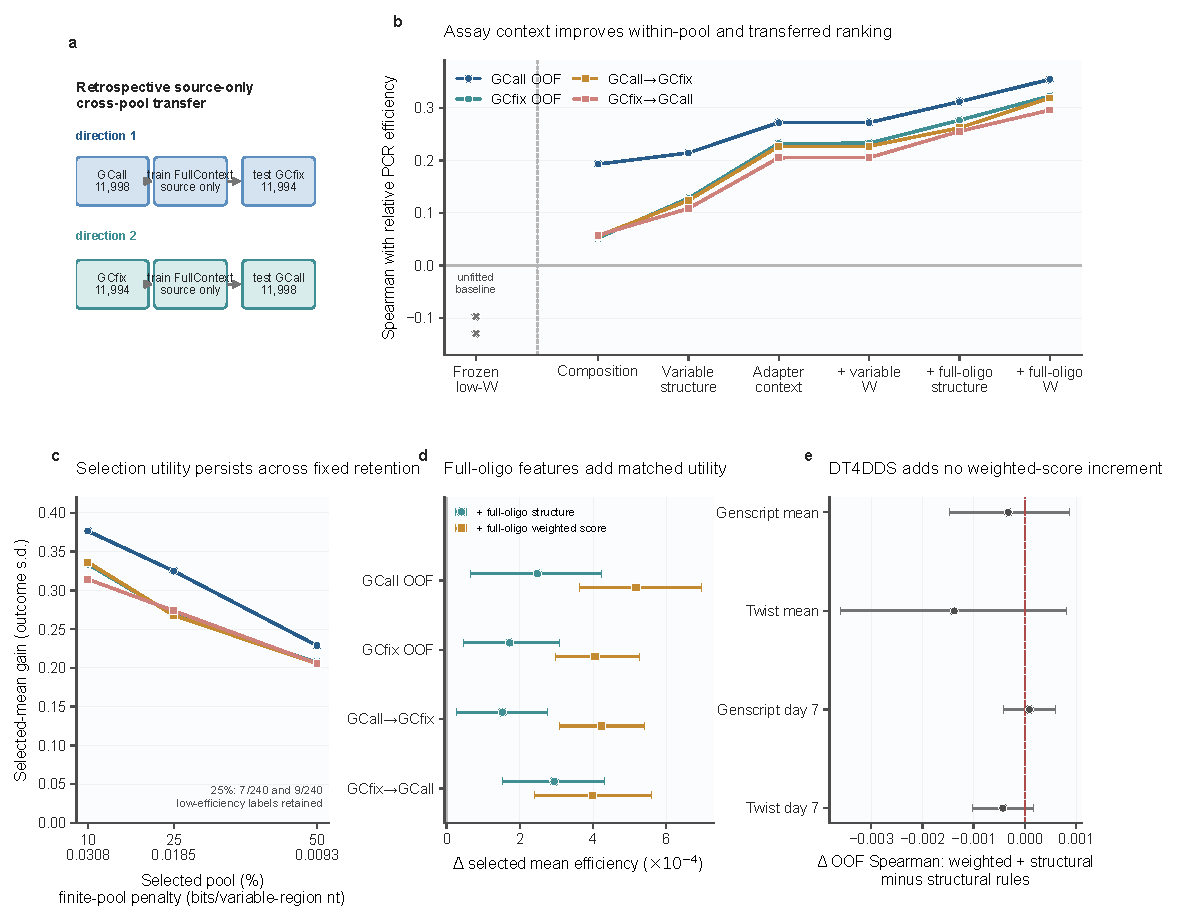
\includegraphics[width=\linewidth]{figures/assay_calibrated_selection.pdf}
\caption{\textbf{Retrospective assay-context modelling in public measured libraries.} (a) Outcome-excluded source-only transfer between GCall ($n=11{,}998$) and GCfix ($n=11{,}994$), with exhaustive fixed-length Hamming audit. (b) Spearman correlation with measured PCR efficiency; F0 is unfitted and P0--P5 are nested ridge models. OOF denotes five repeated nested five-fold predictions. (c) Measured retained-set gains. (d) Paired 25\%-retention increments from complete-oligonucleotide features; whiskers are percentile 95\% intervals from 2,000 sequence bootstraps without model refitting. Intervals condition on published sequence-level outcomes and exclude assay-measurement uncertainty. (e) Null change in measured DT4DDS abundance ranking. Public sequences were not codec outputs; no panel is prospective emitted-sequence PCR.}
\label{fig:assay-selection}
\par\small\noindent\textbf{Alt text:} A five-panel analysis separates source and target PCR pools, shows their exhaustive sequence-distance audit, compares model ranking and retrospective retained-set gains, and shows a null DT4DDS domain-boundary result.
\end{figure}

\subsection{Retrospective measured selection in cross-pool and external KAPA fibers}

On retrospective GCall/GCfix fibers, FullContext had positive measured contrasts at both widths (Fig.~\ref{fig:choice-codec}b; Supplementary Tables S8--S10). At primary $r=2$, raw gains were 0.002349 and 0.002135, or 0.250 and 0.274 target SDs. FullContext-minus-released-1D-CNN regression intervals were positive for continuous efficiency in all four direction--width comparisons, an endpoint-specific result rather than general model superiority. The published hard rule mostly became a pass/fail tie after stricter eligibility; three of four intervals crossed zero and one was negative (Supplementary Table S8).

The analysis-plan-locked external KAPA codebook also gave positive FullContext selection (Fig.~\ref{fig:choice-codec}c): standardized gains were 0.234--0.390 for the GCall-trained selector and 0.229--0.327 for the GCfix-trained selector. These already-public measurements came from an external laboratory in the same source publication, not independent third-party replication. Continuous-efficiency FullContext-minus-CNN intervals were positive, but all endpoint-matched low-efficiency risk-difference intervals included zero. Comparisons with released 1D-CNN outputs were therefore endpoint-dependent. Thirty-two post hoc outcome-blind mappings supported grouping stability but were not experimental repeats (Supplementary Tables S15, S16 and S20).

The corresponding absolute FullContext gains were modest (0.0021--0.0041 on the published relative-efficiency scale). Their practical relevance should be interpreted jointly with standardized effects, low-efficiency event risk and prospective synthesis-level validation.

All eight matched-condition FullContext intervals were positive after source and target resampling (Fig.~\ref{fig:choice-codec}d), and all primary gains were inconsistent with random within-fiber selection under the prespecified procedure (full tests in Supplementary Information). Benefit was not uniform: 17.2--30.9\% of fibers were negative, extremes were $-0.053307$ to 0.058929, and 0.8--4.7\% were within 0.01 target SD of zero. Post hoc score-margin abstention did not eliminate negative fibers and is not a validated safety rule.

The secondary exploratory Q5 workflow-shift sensitivity reversed the external KAPA result. FullContext raw gains ranged from $-0.018596$ to $-0.003785$, 47.7--71.9\% of fiber gains were negative and all four source-plus-target intervals were below zero. At $r=4$, selected low-efficiency event rates rose from a random-choice expectation of 0.0186 to 0.0625 for both source models. Score-margin abstention did not restore positive mean gain. This negative boundary is consistent with assay-conditional rather than polymerase-universal transfer.

\subsection{Computational verification and predicted rate--score trade-off in the generated language}

Independent recurrences returned the same exact 108-nt language size, and explicit length-8 enumeration round-tripped all 45,128 ranks. The fixed base map carries 213 bits (1.9722 bits per variable-region nucleotide). Reserving $r=2$ or $r=4$ leaves 211 bits (1.9537) or 209 bits (1.9352) per variable-region nucleotide. All 65,024 generated candidates passed rank, inverse-modulo-$N$ and payload checks. Exact-language ranks whose inverse lay outside $[0,M)$ and invalid constrained sequences failed closed; a valid noncanonical candidate remained payload-decodable and was rejected only by the optional canonical verifier (Fig.~\ref{fig:choice-codec}a).

Across $r=0,\ldots,6$, retained payload decreased from 213 to 207 bits while generated FullContext mean score gain rose from 0 to 0.004720 (GCall model) and 0.005098 (GCfix model; Fig.~\ref{fig:choice-codec}e). These are predictions, and own-model nonnegative gain partly follows from score maximization. The modulo-$N$ map avoided the first-base exclusion induced by a power-of-two lexicographic prefix: first-base frequencies were 0.2496--0.2503 and all positional base frequencies were 0.2369--0.2618. Eight outcome-blind namespaces had positive predicted gains and no round-trip failure, but no mapping is claimed optimal. Complete domain-shift and runtime diagnostics are in Supplementary Tables S22--S24; none converts predictions into measured PCR evidence.

\begin{figure}[t]
\centering
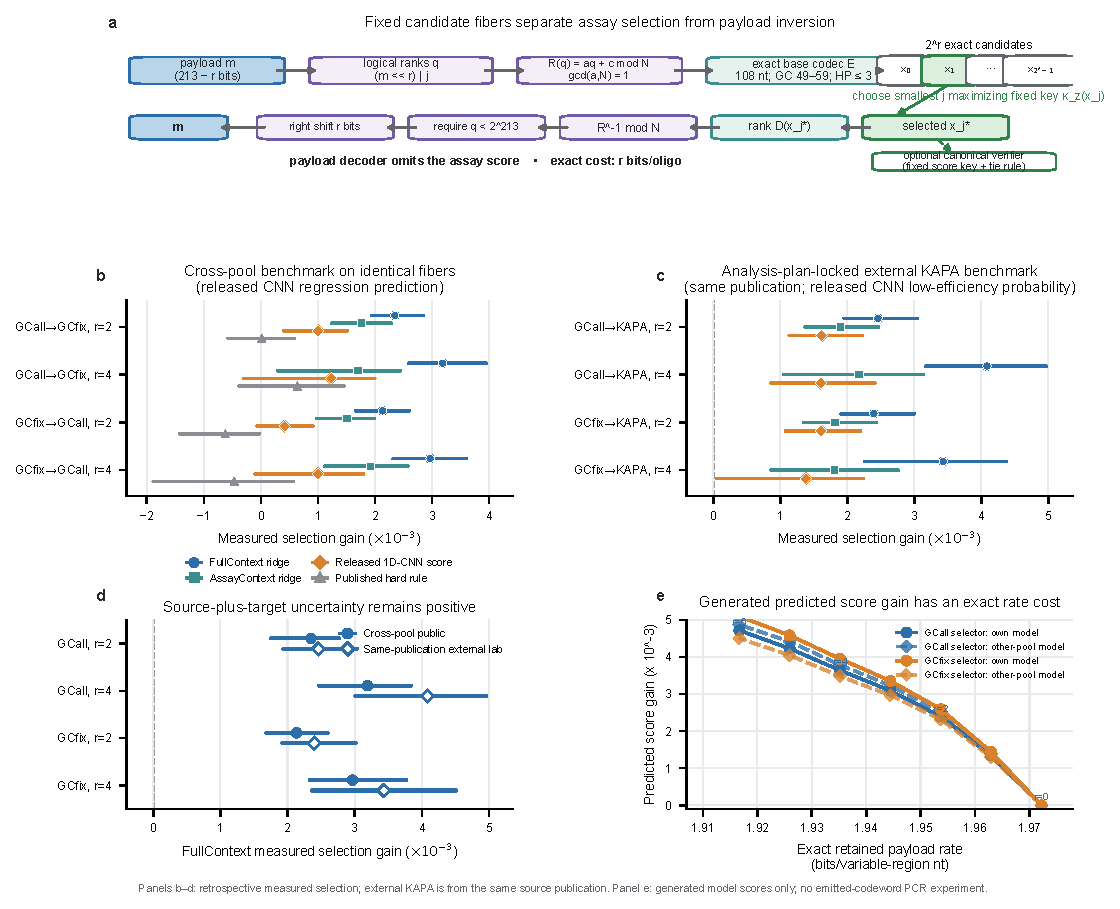
\includegraphics[width=\linewidth]{figures/reversible_choice_codec.pdf}
\caption{\textbf{Exact reversible choice coding and retrospective assay-guided selection.} (a) Full-language modulo-$N$ choice coding and scorer-independent payload inversion. (b,c) Retrospective measured selected-minus-fiber-mean PCR-efficiency gains on fixed GCall/GCfix and external-KAPA fibers; released CNN endpoints differ. Whiskers are marginal 95\% BCa intervals from 2,000 target-fiber resamples. (d) Grouped-source plus target-fiber two-stage 95\% intervals show positive matched-assay gains and negative secondary exploratory Q5 gains on a common zero axis. All intervals condition on published sequence-level outcomes and exclude technical-replicate, batch, normalization and assay-measurement uncertainty. (e) Predicted generated-codeword score--rate trade-off per 108-nt variable region. Generated candidates were computationally verified but not synthesized or assayed. Complete definitions and intervals are in Supplementary Information.}
\label{fig:choice-codec}
\par\small\noindent\textbf{Alt text:} A method schematic separates score-independent payload inversion from optional canonical verification. Forest plots compare retrospective measured outcomes selected by FullContext, AssayContext, released endpoint-specific 1D-CNN outputs and a hard rule. A shared-zero forest plot shows positive cross-pool and external-KAPA intervals but negative exploratory Q5 altered-protocol intervals. A final line plot shows only predicted generated-sequence score--rate trade-offs.
\end{figure}

A separate DT4DDS replay found no improvement from adding the variable-region weighted pair count to composite abundance ranking; all intervals included zero (Fig.~\ref{fig:assay-selection}e; Supplementary Table S28). This negative boundary prevents treating that statistic as a universal molecular-risk direction.

\section{Discussion}

Choice fibers provide a narrow fixed-rate shaping/list-selection interface for an exact oligonucleotide codec. Enumerative constrained coding, rejection sampling, trellis/list shaping and model-based screening establish the individual ingredients as prior art \cite{cover1973enumerative,erlich2017dnafountain,forney1992trellisshaping,wu2022listccdm}. Recent graph-based constrained codecs, indel-aware designs, system simulators and standardized recovery benchmarks are compared in the Supplementary prior-art matrix. The contribution here is the combined semantic contract: globally defined disjoint fibers, fixed candidate and $r$-bit budgets, scorer-free payload inversion, scorer-replacement invariance, separate canonical verification and identical-fiber evaluation with measured PCR outcomes. We do not claim to have introduced constrained coding, representative selection or error correction; the single-edit/CRC audit only documents compatibility with a separate integrity layer.

Model comparisons and transfer were assay- and endpoint-specific. FullContext selected larger continuous mean efficiency than the released scores on the declared fibers, but endpoint-matched FullContext-minus-CNN low-efficiency intervals included zero. The hard rule result likewise reflects a preconstrained codebook, not general filter inefficacy. More importantly, changing from KAPA to Q5 reversed mean gains and yielded 47.7--71.9\% negative fibers. A selector calibrated for one polymerase, temperature and workflow is not an intrinsic sequence-quality function; a new protocol requires empirical recalibration or retraining. Coding correctness remains assay-independent, whereas utility does not.

The external KAPA outcomes were already public when the dated local analysis plan was applied. The pool was measured in another laboratory but reported in the same source publication and was not emitted by this codec. It is neither third-party replication nor prospective emitted-codeword validation. Generated candidates establish language membership, rate, inversion, mapping sensitivity and predicted scores only; own-model gain partly follows from maximization. Only synthesis and assay can test measured benefit.

Computational determinism also differs from biological reproducibility. Integer maps, fixed score keys, tests and manifests make the software path auditable, not PCR effects invariant to laboratory or reagents. Two-stage intervals include source refitting and target-fiber sampling but remain conditional on final feature families, model class, endpoints, filters and mappings. Mapping namespaces are sensitivity settings, not experimental replicates or evidence of optimality.

The scope is assay-guided PCR selection. Coefficients are associational; the language controls whole-sequence GC count and homopolymers but not synthesis errors, degradation, sequencing errors, hairpins, nanopore bias or long-term stability. We report no NUPACK calculation, material structure assay, emitted-codeword PCR, synthesis, sequencing, file recovery or end-to-end density comparison. A closure experiment should preregister the assay and endpoints, synthesize emitted and baseline members of matched $r=0,2$ (preferably $4$) fibers, and analyse payload/fiber-level amplification and low-efficiency outcomes. Thus the exact construction is model- and assay-independent, but its biological benefit is assay-dependent and awaits prospective validation.

\section*{Availability and implementation}

Code, frozen derived data, tests, figure source data, environments and manifests are public at \url{https://github.com/nessajzhang/exact-reversible-choice-coding} under the BSD-3-Clause licence. Separate commands verify integrity, reproduce analyses and figures, and compile the manuscript. A persistent URL or identifier for a repository-matched archived snapshot will be inserted before formal submission; a DOI is one possible route.

\section*{Data availability}

The PCR inputs, same-publication external-laboratory pools and published comparator outputs are available with Gimpel \emph{et al.} \cite{gimpel2025pcrbias}, including accession PRJEB77604 and the associated repository. DT4DDS inputs are available with Gimpel \emph{et al.} \cite{gimpel2023digitaltwin}. Author-derived frozen tables required for every reported value are public with the code; upstream data remain under their original access and licence terms. Creation of a persistent repository-matched archive remains an author-controlled publication action.

\begingroup
\footnotesize
\bibliographystyle{plain}
\bibliography{references}
\endgroup

\end{document}
